
\section{Loop Antenne}\label{sec:LoopAntenneTheorie}
%%%%%%%%%%%%%%%%%%%%%%%%%%%%%%%%%%%%%%%%%%%%%%%%%%%%%%%%%%%%%
\begin{figure}[h]
	\centering
	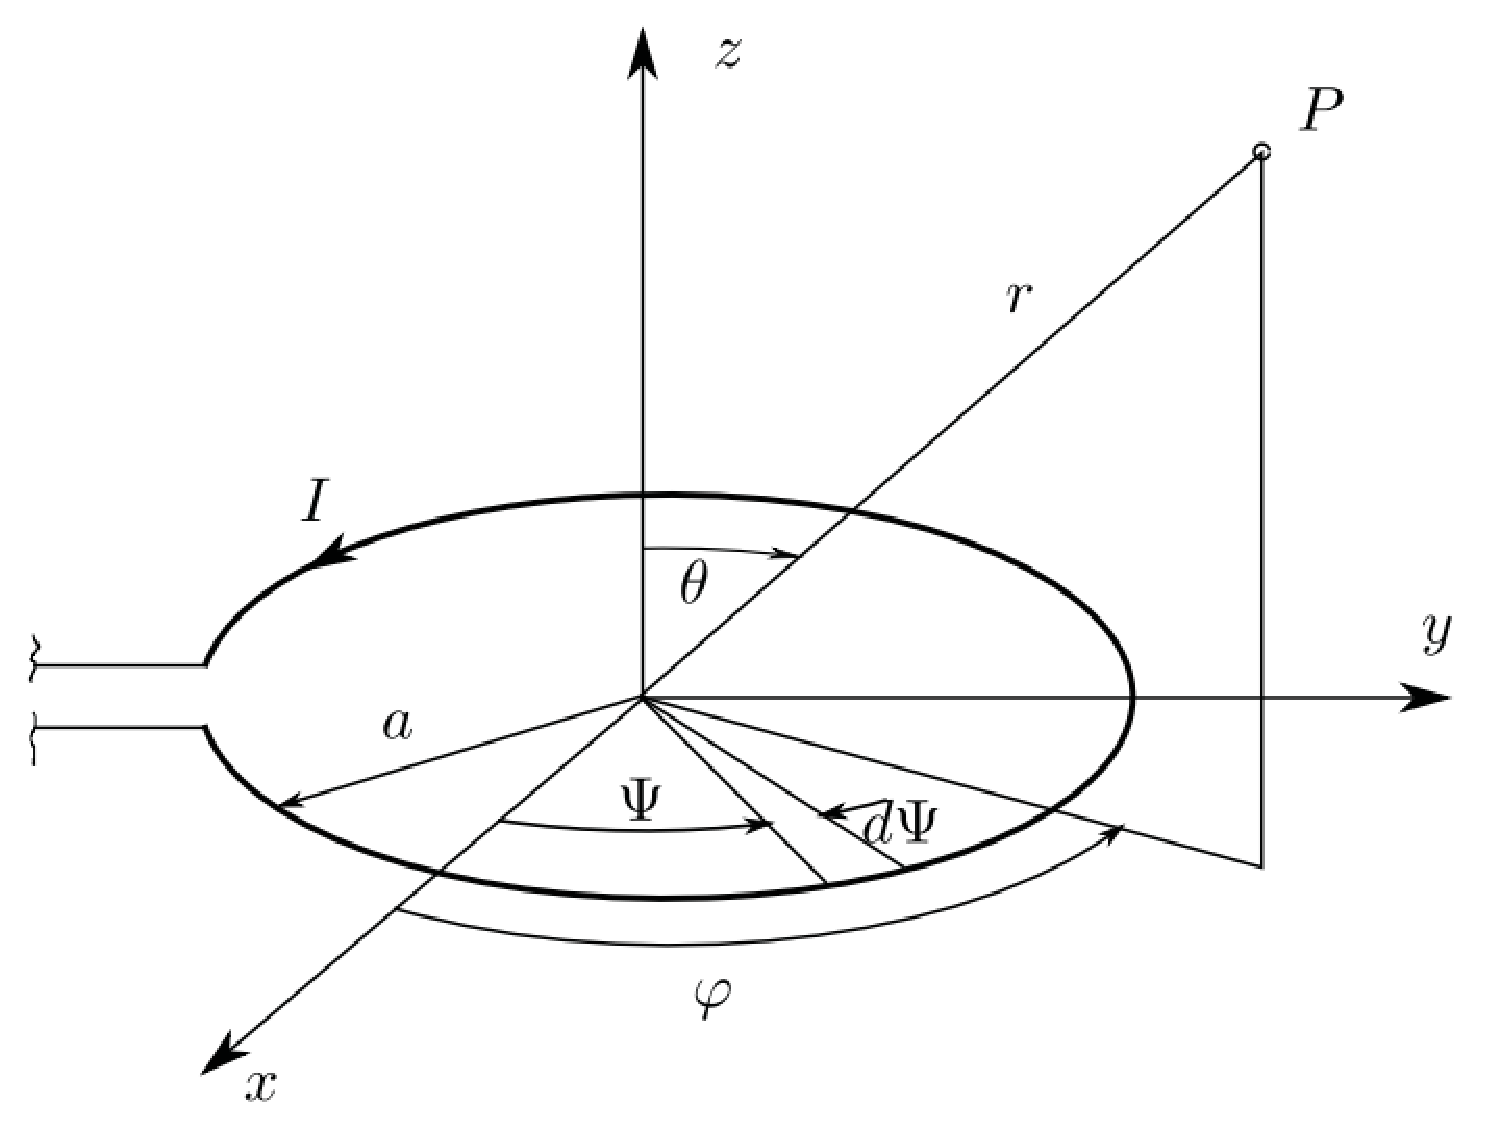
\includegraphics[width=7cm]{content/bilder/Loop_EMANT_S45.pdf}%
	\caption{Loop Antenne}
	\label{LoopAntenne}
\end{figure}
%%%%%%%%%%%%%%%%%%%%%%%%%%%%%%%%%%%%%%%%%%%%%%%%%%%%%%%%%%%%%
Wird eine kurze, kreisförmige Stromschleife mit dem Radius $a<<\lambda$ von einem Strom $Ie^{j\omega t}$ durchflossen, kann in guter Näherung eine konstante Stromverteilung I entlang der Schlaufe angenommen werden. Die Koordinaten eines Punktes auf der Stromschleife sind gegeben mit:
\begin{eqnarray}
x’ &=& a \cos(\Psi)\\
y’ &=& a \sin(\Psi)\\
z’ &=& 0\label{SchlaufeInDerEbene}
\end{eqnarray}
Aus  (\ref{SchlaufeInDerEbene}) wird deutlich, dass die Leiterschleife nur in der xy-Ebene liegt und keine Ausdehung in z-Richtung besitzt. Der Abstand a entspricht dem Radius der Leiterschleife. Der Stromfluss in einem sehr kurzen Leiterstück kann Somit kann beschrieben werden als:
\begin{equation}
I dl= Ia(- \vec e_{x}sin(\Psi)+\vec e_{y}cos(\Psi))d\Psi
\end{equation}
 %EMANT Joss Seit 45
Die Stromverteilung führt zu einer Abstrahlung von elektromagnetischen Wellen. Die Abstrahlung kann mit der Gewichtungsfunktion in Abhänigkeit von $\theta$ und $\varphi$ beschrieben werden. Die ausfühliche Gewichtungsfunktion einer Stromschleife hat R. Elliott \cite{elliott1981antenna} beschrieben. Da die Integration eines geschlossenen Kreises Null ergibt, kann die Gewichtungsfunktion a$\theta(\theta, \varphi)$, abhängig von $\theta$ und $\varphi$, wie folgt vereinfacht werden \cite{Emant}:
%Die Gewichtungsfaktoren findet man mit Hilfe von (116 Joss) und (117 Joss) zu
%Emant Joss Seite 46
%Emant Joss Seite 46
\begin{equation}\label{GewichtungsfunktionLoop_aTheta}
a\theta(\theta, \varphi) =0
\end{equation}
Das Fernfeld ist $\varphi$ polarisiert, da die Gewichtungsfunktion $a\theta$ gleich Null ist. Nimmt man an, dass $ka$ klein ist, so kann die Gewichtungsfunktion $a\varphi$ weiter vereinfacht werden:
%\begin{equation}
%a\varphi(\theta, \varphi)=sin(ka sin(\theta)cos(\psi))=ka sin(\theta)cos(\psi)
%\end{equation}
%dank der Fereinfachung kann xxxx als geschrieben werden.
\begin{equation}
a\varphi(\theta,\varphi)=j(\pi a^{2}I)(k sin \theta)
\end{equation}
%$a(theta, phi)=j$... oder Ellito 2.31 oder Joss Seite 46.
Die Leistungsdichte eines elektromagnetischen Feldes kann mit der allgemeinen Formel (\ref{eq:Leistungsdichte_E_H}) beschrieben werden: 

%(Joss 118) 
\begin{equation}
P(\theta,\varphi)=\frac{1}{2}Re(E x H^*)
\label{eq:Leistungsdichte_E_H}
\end{equation}
zu
%Joss EMANT P(theta,phi)=....Ellito 2.32
\begin{equation}
P(\theta)=\frac{(ka)^{4}I{2}\eta}{32r^{2}}sin^{2}\theta
\end{equation}
Im Vergleich mit dem kurzen Dipol erzeugt die kleine Stromwindung ein vergleichbares Richtdiagramm. Das Fernfeld des kurzen Dipols ist jedoch vertikal $\theta$ polarisiert. Das bedeutet, dass das Abstrahlverhalten um $90^\circ$ verschoben ist. Integriert man die Leistungsdichte über eine Kugeloberfläche mit dem Radius $r$  und setzt sie der abgegebenen Leistung mit $1/2 I^{2}Rrad $ der zugeführten Zweidrahtleitung gleich, so gewinnt man $R_{rad}$:
\begin{equation}
R_{rad} = 320\pi^{6} (a/\lambda)^{4}\label{eq:RradLoop}
\end{equation}
%ELLITOH 2.33
Beispiel:\\
Wenn $a/\lambda = 0.03$ ist, dann wird der $R_{rad} = 0.25\Omega$. Als Vergleich mit dem kurzen Dipol mit der Länge $2l=\lambda= 0.06$ führt das zu einem Strahlungswiderstand $R_{rad}$ von $0.7\Omega$.  Der Abstrahlwiderstand $R_{rad}$ einer kleinen Stromschleife kann um den Faktor $n^{2}$ erhöht werden, wenn n die Anzahl der sehr eng aneinander liegenden Wicklungen der Stromschleife sind. 



%%%%%%%%%%%%%%%%%%%%%%%%%%%%%%%%%%%%%%%%%%%%%%%%%%%%%%%%%%%%%
\begin{figure}[h!]
\begin{center}
\begin{tikzpicture}
	\draw (0,3)  -- (10,3);
	\draw (5,0) -- (5,6);%Fadenkreuz vertikal
	\draw (3,3) circle (2cm);%linker Kreis
	\draw (7,3) circle (2cm);%rechter Kreis
	\draw (4.5,3) circle (0.2cm);%linker kleiner Kreis
	\draw (5.5,3) circle (0.2cm);%rechter kleiner Kreis
	\draw (4.5,3.2) -- (5.5,3.2);%Verbindung horizontal oben
	\draw (4.5,2.8) -- (5.5,2.8);%Verbinung horizontal unten
	\draw[line width=0.4pt, ->, >=latex](5, 5) -- (5, 6.1) node at (4.5,6){z};
	\draw[line width=0.4pt, ->, >=latex](9, 3) -- (10.1, 3) node at (10.5,3){x};
	\node[draw] at (5,6.5) {$\theta=0 ^\circ$};
	\node[draw] at (8,5.5) {$E_{\varphi}(\theta)$};
	
	%%%%%%
	%vetor Pfeil
		\draw[line width=0.4pt, ->, >=latex](5, 3) -- (7, 5) node at (7,4.7){$\vec{r}$};

	\coordinate (A) at (5, 5.5);
	\coordinate (B) at (6.4, 4.5);
	\coordinate (a) at (5.6, 5.4);
	\draw[line width=0.5pt, dashed, very thick,cap=round,->](A) .. controls (a) .. node[above] {$\theta$} (B);
\end{tikzpicture}
\end{center}
\caption{E-Feld einer Loop Antenne in der xz-Ebene}
\label{DipolEFerd}
\end{figure}
%%%%%%%%%%%%%%%%%%%%%%%%%%%%%%%%%%%%%%%%%%%%%%%%%%%%%%%%%%%%%